% main.tex
% Fichero principal de transparencias (incluye a todos los demás).

% Compilar a .pdf con LaTeX (pdflatex)
% Es necesario instalar Beamer (paquete latex-beamer en Debian)
%

% Gráficos:
% Los gráficos pueden suministrarse en PNG, JPG, TIF, PDF, MPS
% Los EPS deben convertirse a PDF (usar epstopdf)
%
\documentclass[17pt,aspectratio=169,hyperref=pdfusetitle]{beamer}
\usetheme[orchid]{Hannover}
\beamertemplatenavigationsymbolsempty
\setbeamertemplate{headline}{}
\useoutertheme{infolines}

\usepackage[spanish]{babel}
\usepackage[utf8]{inputenc}
\usepackage{graphics}
%\usepackage{amssymb} % Simbolos matematicos
%\usepackage[pdfusetitle]{hyperref}

\usepackage{chronosys}

%% two slides per page
%\usepackage{pgfpages}
%\pgfpagesuselayout{2 on 1}[a4paper,border shrink=5mm]

\newcommand\YUGE{\fontsize{48}{60}\selectfont}

\newcommand{\secimage}{figs/bookpages}
\AtBeginSection[]
{
  {
    \usebackgroundtemplate{\includegraphics[width=\paperwidth,height=\paperheight]{\secimage}}
    \begin{frame}<beamer>

      \begin{center}
        {\YUGE\bf\insertsection}
      \end{center}
    \end{frame}
  }
  \renewcommand{\secimage}{figs/bookpages}
}


\title[Learning from errors]{Learning from errors: \\ my academic career}
%\subtitle{}
\author[Jesus M. Gonzalez-Barahona]{Jesus M. Gonzalez-Barahona}
\institute[URJC]{Universidad Rey Juan Carlos \\
  @jgbarah ~~~~~ \url{http://github.com/jgbarah/presentations}}

\date[ICSME Doctoral Symposium]{ICSME Doctoral Symposium \\ Madrid (Spain), September 25th 2018}

\begin{document}

%\begin{frame}[label=firstframe]
\begin{frame}
  \maketitle
\end{frame}


\begin{frame}

  {\em
    \begin{center}
      %\begin{quote}
      ``Once upon a time \\
      there was a wannabe researcher \\
      in the Deep South of Madrid...''\\
      %\end{quote}
    \end{center}
  }
\end{frame}


%%%%%%%%%%%%%%%%%%%%%%%%%%%%%%%%%%%%%%%%%%%%%%%%%%%%%%%%%%%%%%%%
%%%%%%%%%%%%%%%%%%%%%%%%%%%%%%%%%%%%%%%%%%%%%%%%%%%%%%%%%%%%%%%%
% lista de temas                                               %
%%%%%%%%%%%%%%%%%%%%%%%%%%%%%%%%%%%%%%%%%%%%%%%%%%%%%%%%%%%%%%%%
%%%%%%%%%%%%%%%%%%%%%%%%%%%%%%%%%%%%%%%%%%%%%%%%%%%%%%%%%%%%%%%%


\definecolor{lightviolet}{HTML}{F4AFF4}
\definecolor{lightorange}{HTML}{FFA17F}
\definecolor{lightgreen}{HTML}{98FB98}
\definecolor{lightred}{HTML}{FF5C5C}
\definecolor{lightblue}{HTML}{89AFCF}
\definecolor{lightbrown}{HTML}{B58868}

%%-----------------------------------------
%%-----------------------------------------
\section{Starting conditions}


%%-----------------------------------------
\begin{frame}[fragile]
  \frametitle{Being in the right place}

  \begin{center}
  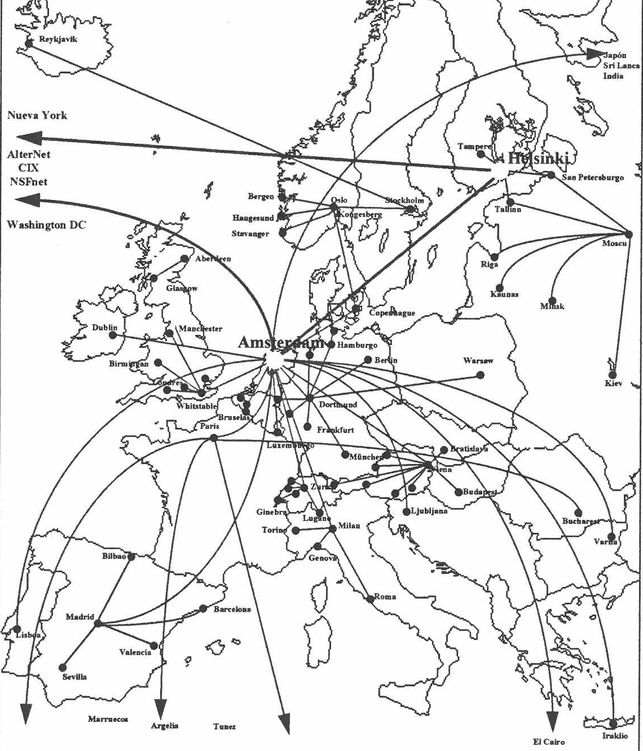
\includegraphics[height=6cm]{figs/eunet}
  \end{center}  
  
\end{frame}

%%-----------------------------------------
\begin{frame}[fragile]
  \frametitle{Being in the right place (lesson)}

  Look for exciting stuff \\
  stuff that will change the world \\
  even it doesn't seem that academic \\
  and understand it \\

    \begin{center}
    Look at the future, we're doing it
    \end{center}

\end{frame}

%%-----------------------------------------
\begin{frame}[fragile]
  \frametitle{Being at the right moment}

  \begin{center}
  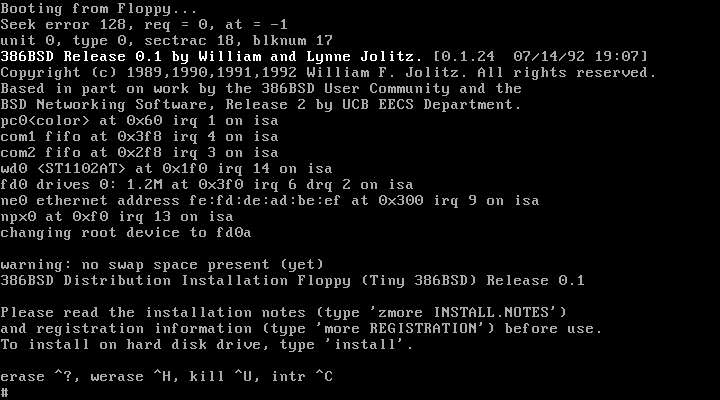
\includegraphics[height=6cm]{figs/386BSD-installer}
  \end{center}  
  
\end{frame}

%%-----------------------------------------
\begin{frame}[fragile]
  \frametitle{Being at the right moment (lesson)}

  Play with cool stuff \\
  Experiment \\
  Build on the work of others \\
  Have fun \\

  \begin{center}
    Learn by doing
  \end{center}
\end{frame}

%%-----------------------------------------
\begin{frame}[fragile]
  \frametitle{Having the right mentors}

  \begin{center}
  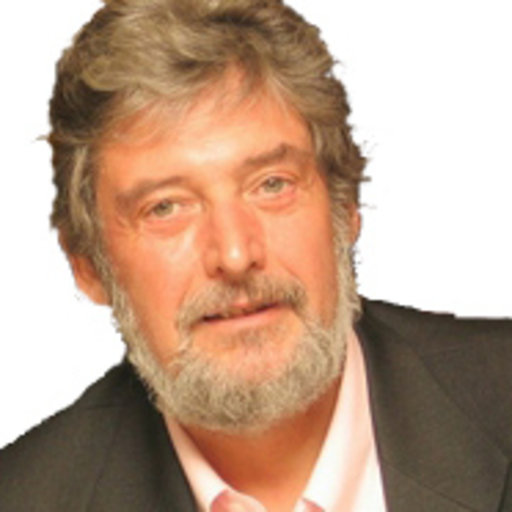
\includegraphics[height=3.5cm]{figs/foto-aalvarez}
  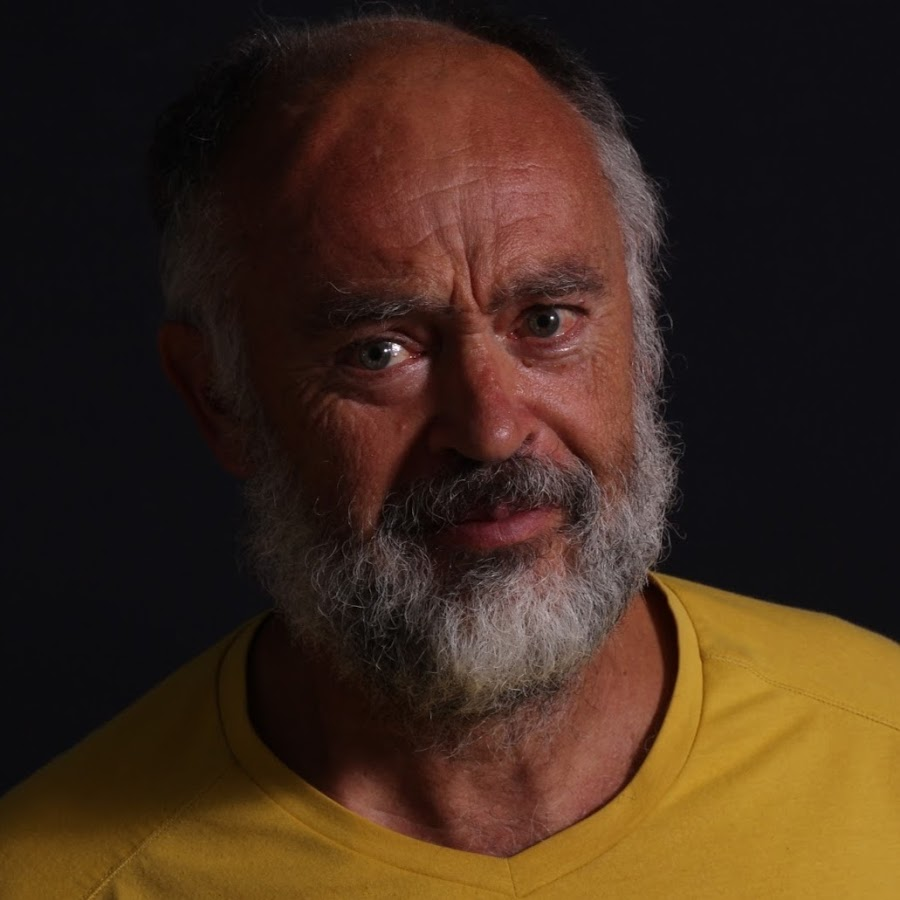
\includegraphics[height=3.5cm]{figs/foto-jseoane}
  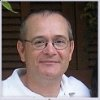
\includegraphics[height=3.5cm]{figs/foto-sarevalo}
  \end{center}  
  
\end{frame}

%%-----------------------------------------
\begin{frame}[fragile]
  \frametitle{Having the right mentors (lesson)}

  Network with interesting people \\
  You understand when you can explain \\
  Details are (very) important \\

  \begin{center}
    Yes, I can \\
    (English skills are fundamental) \\
  \end{center}
\end{frame}

%%-----------------------------------------
\begin{frame}[fragile]
  \frametitle{Having the right colleagues}

  \begin{center}
  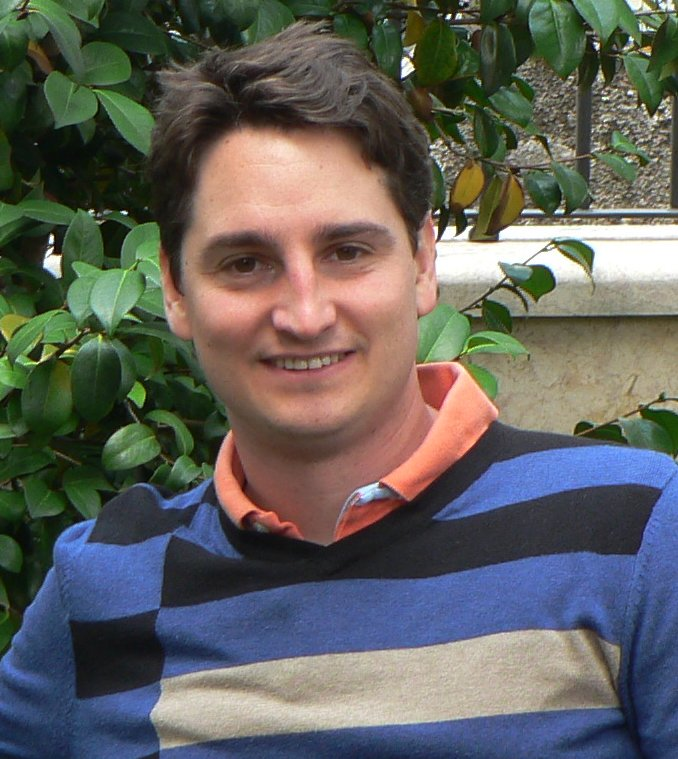
\includegraphics[height=4.5cm]{figs/gregorio-robles}
  \end{center}  
  
\end{frame}

%%-----------------------------------------
\begin{frame}[fragile]
  \frametitle{Having the right colleagues (lesson)}

  Having great people around is very important \\
  Playing in a team is much more fun \\
  Together you can reach higher \\
  
  \begin{center}
    Let's try it
  \end{center}  
  
\end{frame}

%%-----------------------------------------
\begin{frame}[fragile]
  \frametitle{Having the path paved}

  \begin{center}
  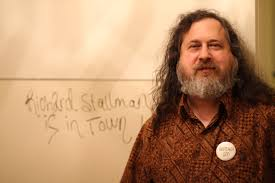
\includegraphics[height=6cm]{figs/foto-rms}
  \end{center}  
  
\end{frame}

%%-----------------------------------------
\begin{frame}[fragile]
  \frametitle{Having the path paved (lesson)}

  The importance of sharing \\
  The importance of ethics \\
  The importance of tools \\

  \begin{center}
    Have principles, but have also a plan
  \end{center}
\end{frame}

%%-----------------------------------------
%%-----------------------------------------
\section{A (very personal) story}


%%-----------------------------------------
\begin{frame}[fragile]
  \frametitle{Labs based on free software (1993-2005)}

  \begin{center}
  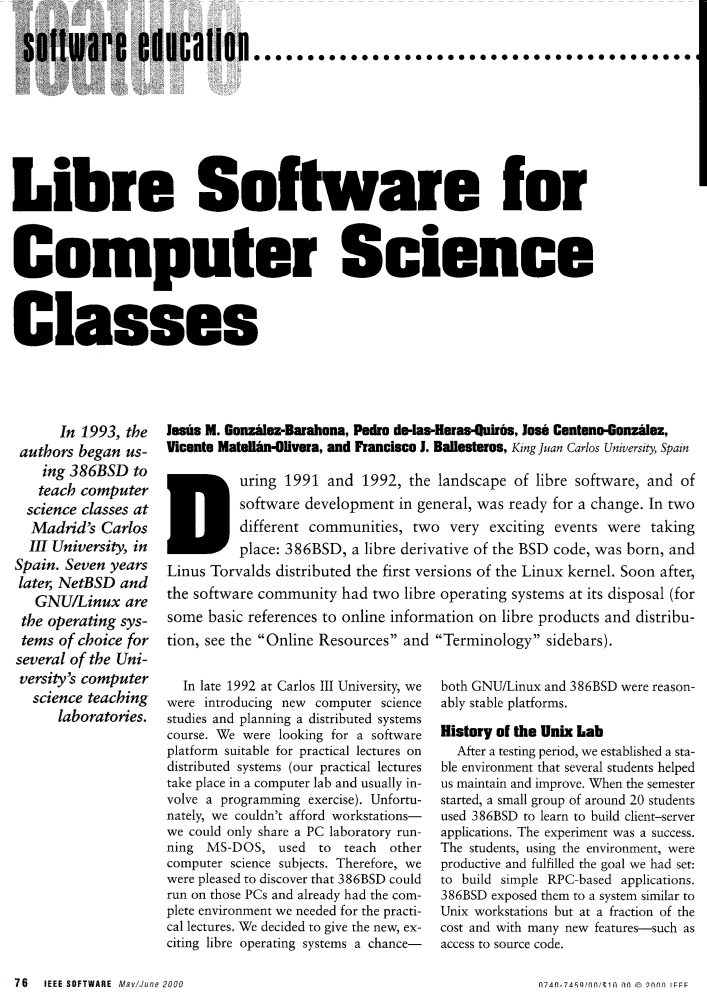
\includegraphics[height=8cm]{figs/libre-classes}
  \end{center}  
  
\end{frame}

%%-----------------------------------------
\begin{frame}[fragile]
  \frametitle{Labs based on free software (lesson)}

  Cool stuff may need a lot of time \\
  a lot \\
  a whole lot \\

  \begin{center}
    But it may pay the effort
  \end{center}  
  
\end{frame}


%%-----------------------------------------
\begin{frame}[fragile]
  \frametitle{PhD thesis \& Lower\_Layer (1995-2002)}

  \begin{center}
  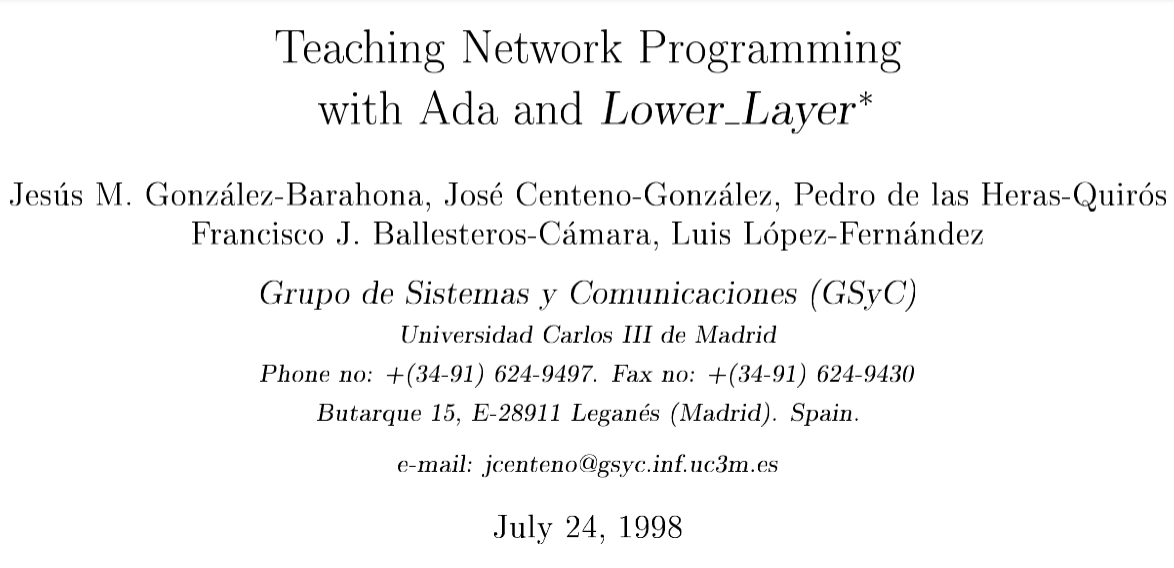
\includegraphics[width=12cm]{figs/lower-layer}
  \end{center}  
  
\end{frame}

%%-----------------------------------------
\begin{frame}[fragile]
  \frametitle{PhD thesis \& Lower\_Layer (lesson)}

  Details are important, \\
  but getting things done too \\
  Doing is important \\
  but focus too \\
  
  \begin{center}
    It's difficult to identify the main result
  \end{center}  
  
\end{frame}

%%-----------------------------------------
\begin{frame}[fragile]
  \frametitle{Free software in Europe (1997-2005)}

  \begin{center}
  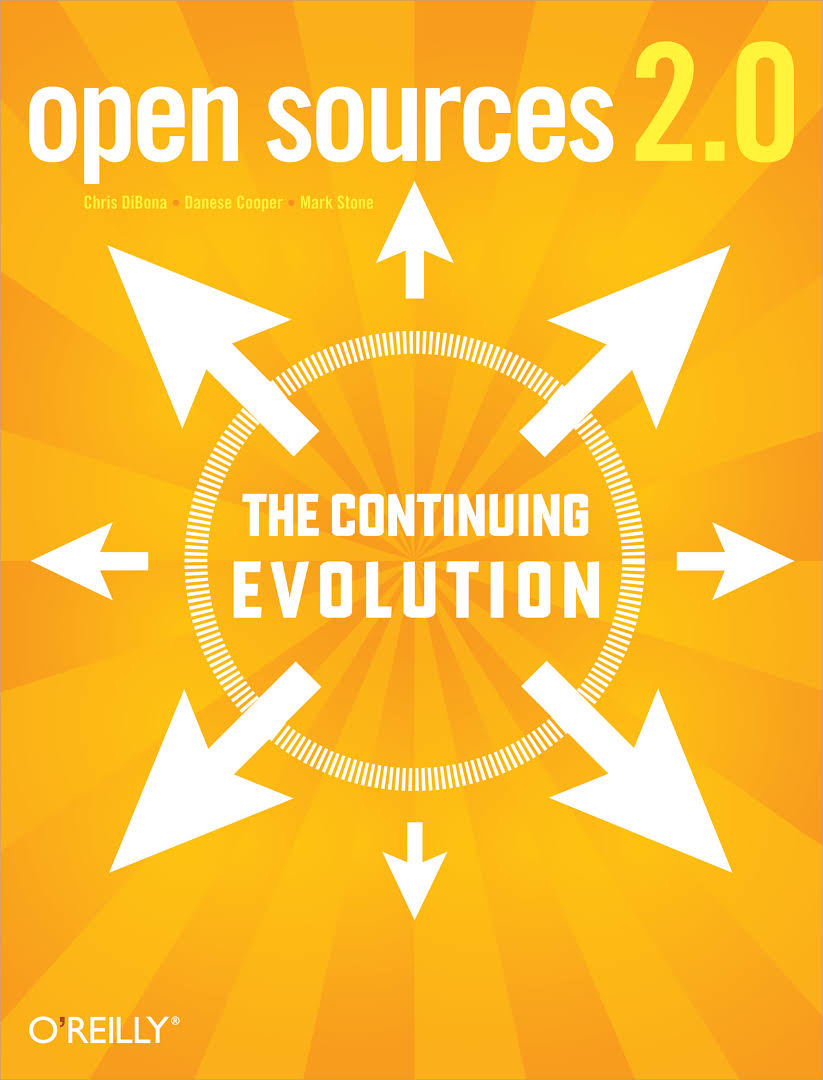
\includegraphics[height=8cm]{figs/opensources}
  \end{center}  
  
\end{frame}

%%-----------------------------------------
\begin{frame}[fragile]
  \frametitle{Free software in Europe (lesson)}

  You can do cool stuff \\
  at many levels \\
  with cool people \\

  \begin{center}
    It may count as zero for your academic life
  \end{center}  
  
\end{frame}


%%-----------------------------------------
\begin{frame}[fragile]
  \frametitle{Counting potatoes (2000-2001)}

  \begin{center}
  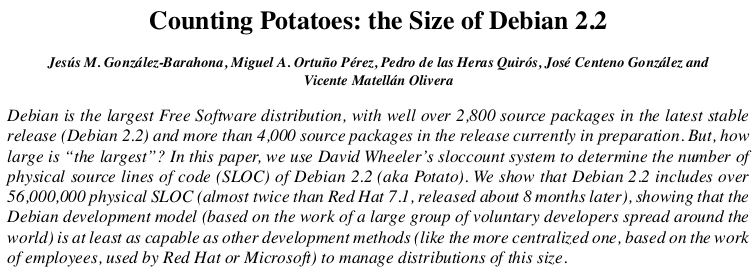
\includegraphics[width=12cm]{figs/counting-potatos}

  
\includegraphics[width=6cm]{figs/upgrade}
  \end{center}  
  
\end{frame}

%%-----------------------------------------
\begin{frame}[fragile]
  \frametitle{Counting potatoes (lesson)}

  Any detail may change a life \\
  In some moments you're ready for a change \\
  and you feel you have been preparing for it \\
  
  \begin{center}
    Switching fields may be rebooting from scratch
  \end{center}
  
\end{frame}

%%-----------------------------------------
\begin{frame}[fragile]
  \frametitle{Using data from CVS (lesson)}

  \begin{center}
  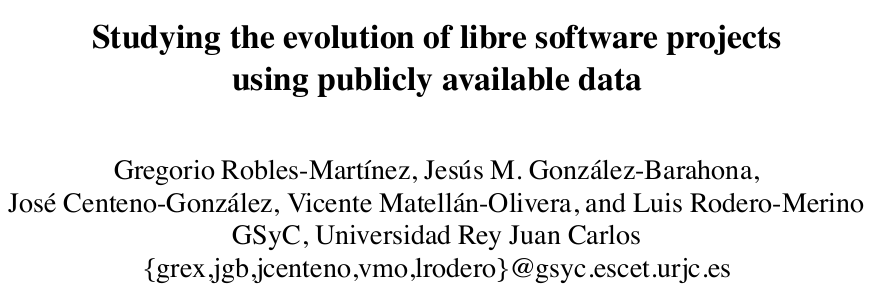
\includegraphics[width=12cm]{figs/evolution-data}
  \end{center}  
  
\end{frame}

%%-----------------------------------------
\begin{frame}[fragile]
  \frametitle{Using data from CVS (2001-2003)}

  The are niches of opportunity \\
  that you can exploit better than others \\
  but quickly you need to learn new stuff \\
  
  \begin{center}
    Starting in a new research field \\
    is not always easy \\
  \end{center}  
  
\end{frame}


%%-----------------------------------------
\begin{frame}[fragile]
  \frametitle{CVSAnalY (2002-2015)}

  \begin{center}
  
\includegraphics[width=12cm]{figs/cvsanaly}
  \end{center}  
  
\end{frame}

%%-----------------------------------------
\begin{frame}[fragile]
  \frametitle{CVSAnalY (lesson)}

  Tools are important and cool \\
  Tools help you learn the details \\
  Tools can be done in collaboration \\
  
  \begin{center}
      Good tools don't guarantee publication
  \end{center}  
  
\end{frame}


%%-----------------------------------------
\begin{frame}[fragile]
  \frametitle{Macro-evolution (2005-2008)}

  \begin{center}
  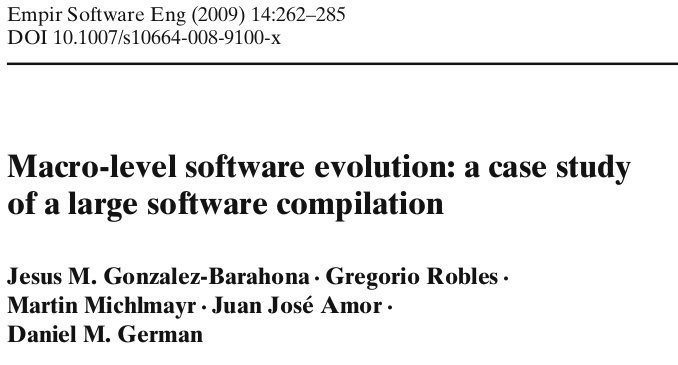
\includegraphics[width=12cm]{figs/macro-evolution}
  \end{center}  
  
\end{frame}

%%-----------------------------------------
\begin{frame}[fragile]
  \frametitle{Macro-evolution (lesson)}

  A solid work may take a little while... \\
  ...with a little help from friends \\
  and your past experience \\
  
  \begin{center}
    But you need to find the right approach
  \end{center}  
  
\end{frame}

%%-----------------------------------------
\begin{frame}[fragile]
  \frametitle{Teaching about free software (2002-2008)}
  
  \begin{center}
  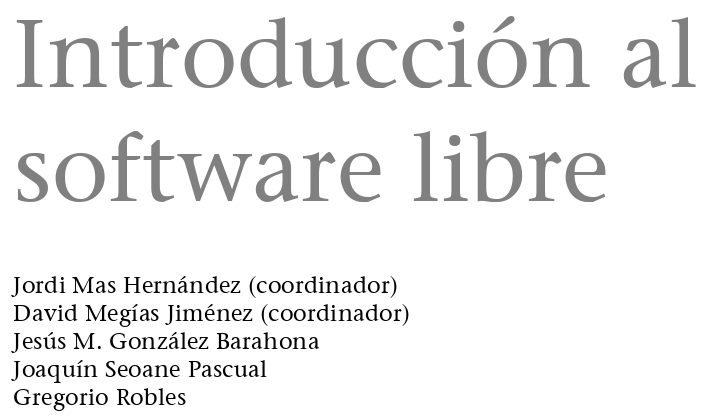
\includegraphics[width=12cm]{figs/intro-sobre}
  \end{center}  
  
\end{frame}

%%-----------------------------------------
\begin{frame}[fragile]
  \frametitle{Teaching about free software (lesson)}
  
  Learning by teaching \\
  Gaining perspective \\
  Observing the landscape \\
  Having a looooot of fun \\
  
  \begin{center}
    Teaching takes a looooot of time
  \end{center}  
  
\end{frame}

%%-----------------------------------------
\begin{frame}[fragile]
  \frametitle{FLOSSMetrics (2006-2009)}

  \begin{center}
  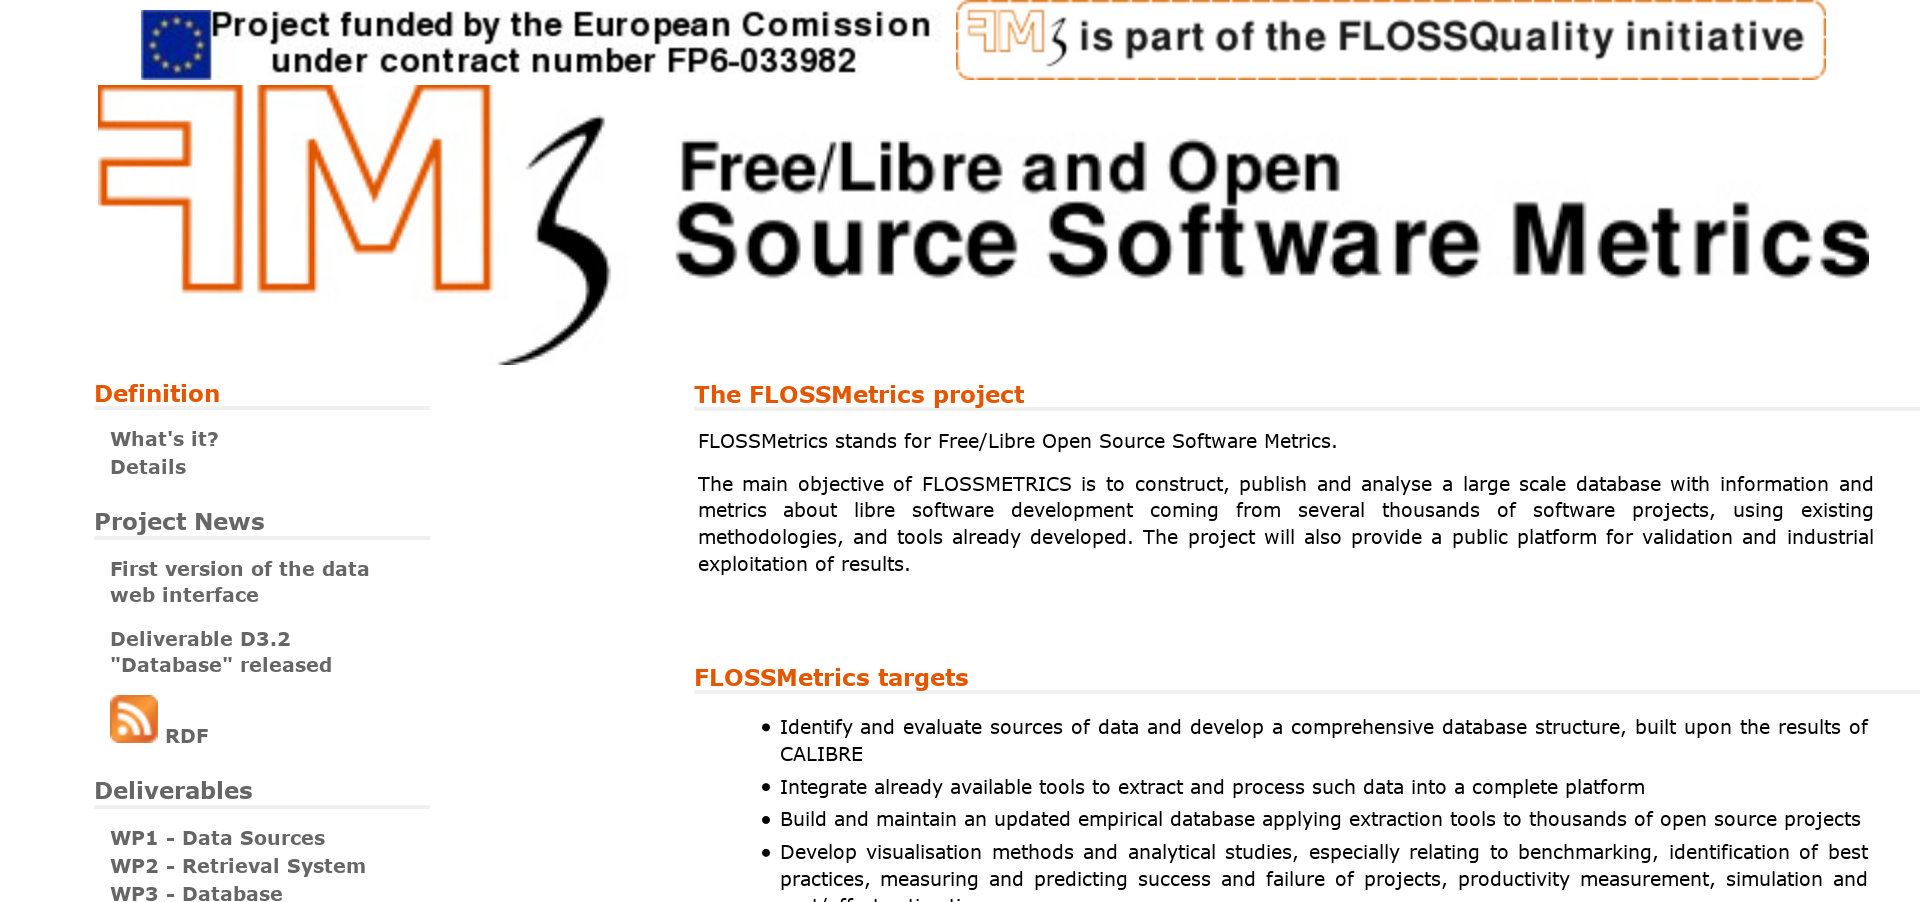
\includegraphics[width=12cm]{figs/flossmetrics}
  \end{center}  
  
\end{frame}

%%-----------------------------------------
\begin{frame}[fragile]
  \frametitle{FLOSSMetrics (lesson)}

  Funded projects bring resources \\
  They allow for implementing ambitious ideas \\
  They put together interesting teams \\
  
  \begin{center}
    Funded projects may be (very) distracting
  \end{center}  
  
\end{frame}

%%-----------------------------------------
\begin{frame}[fragile]
  \frametitle{Studying Wikipedia (2007-2009)}

  \begin{center}
  
\includegraphics[width=12cm]{figs/wikipedia}
  \end{center}  
  
\end{frame}

%%-----------------------------------------
\begin{frame}[fragile]
  \frametitle{Studying Wikipedia (lessons)}

  You can explore new fields \\
  with some advantage \\
  because you have the right background \\
  and the right people around \\
  
  \begin{center}
    Did I say that new fields may be like \\
    rebooting from scratch? \\
  \end{center}  
  
\end{frame}

%%-----------------------------------------
\begin{frame}[fragile]
  \frametitle{Reproducibility (2008-2012)}

  \begin{center}
  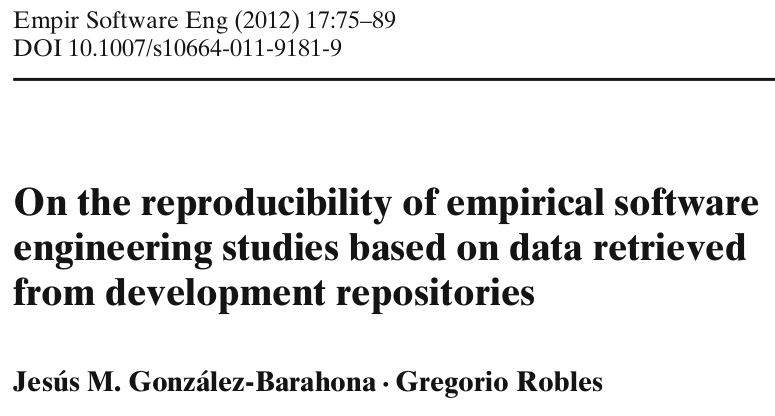
\includegraphics[width=12cm]{figs/reproducibility}
  \end{center}  
  
\end{frame}

%%-----------------------------------------
\begin{frame}[fragile]
  \frametitle{Reproducibility (lesson)}

  You can step back for a moment \\
  look at things from a new perspective \\
  and find a new use for what you know \\
  
  \begin{center}
    Literature surveys may be fun, but hard too
  \end{center}  
  
\end{frame}

%%-----------------------------------------
\begin{frame}[fragile]
  \frametitle{Evolution based in data (2008-2013)}

  \begin{center}
  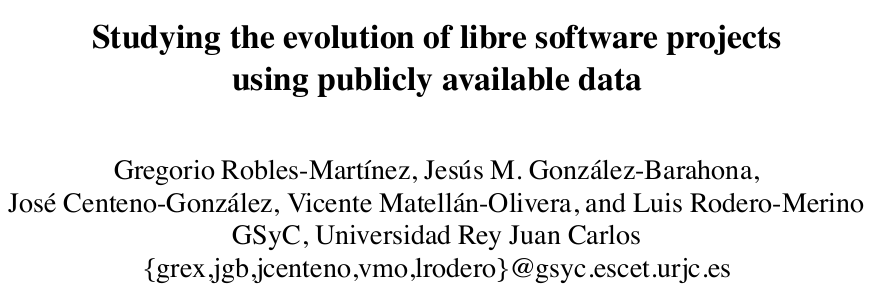
\includegraphics[width=12cm]{figs/evolution-data}
  \end{center}  
  
\end{frame}

%%-----------------------------------------
\begin{frame}[fragile]
  \frametitle{Evolution based in data (lesson)}

  Reproducing past research is fun \\
  and interesting \\
  and helps to advance the state of the art \\
  It may lead to new lines \\
  
  \begin{center}
    Reproducing is not always easy
  \end{center}  
  
\end{frame}

%%-----------------------------------------
\begin{frame}[fragile]
  \frametitle{Companies and communities (2010-2013)}

  \begin{center}
  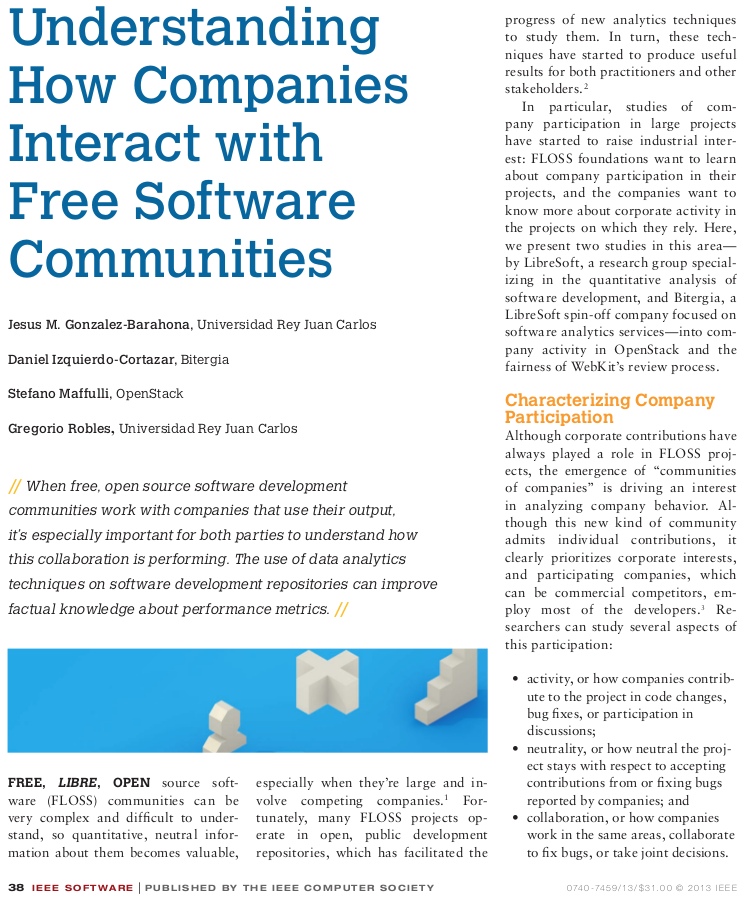
\includegraphics[width=12cm]{figs/software-companies}
  \end{center}  
  
\end{frame}

%%-----------------------------------------
\begin{frame}[fragile]
  \frametitle{Companies and communities (lesson)}

  The real world is there, and it's nice \\
  If you can explain a part of it \\
  that will be appreciated \\
  
  \begin{center}
    The real world is dirty, complex, \\
    difficult to understand \\
  \end{center}  
  
\end{frame}

%%-----------------------------------------
\begin{frame}[fragile]
  \frametitle{MetricsGrimoire (2002-2015)}

  \begin{center}
  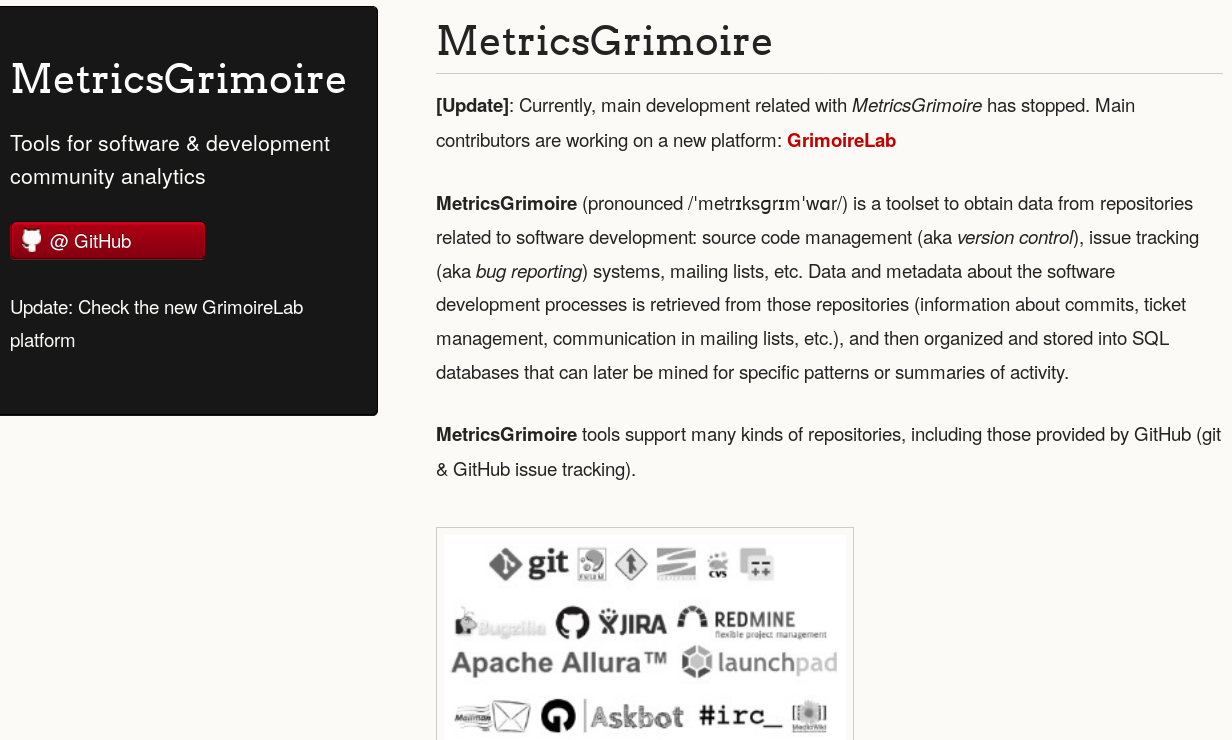
\includegraphics[width=12cm]{figs/metricsgrimoire}
  \end{center}  
  
\end{frame}

%%-----------------------------------------
\begin{frame}[fragile]
  \frametitle{MetricsGrimoire (lesson)}

  Tools keep you anchored in reality \\
  Tools give you a competitive advantage \\
  Tools let you learn the details \\
  
  \begin{center}
    Tools may be distracting, \\
    difficult to ``convert'' in papers \\
  \end{center}  
  
\end{frame}

%%-----------------------------------------
\begin{frame}[fragile]
  \frametitle{Bitergia (2012-)}

  \begin{center}
  
\includegraphics[width=12cm]{figs/bitergia}
  \end{center}  
  
\end{frame}

%%-----------------------------------------
\begin{frame}[fragile]
  \frametitle{Bitergia (2012-)}

  Startups are a lot of fun \\
  They link you to reality, \\
  and see a new side of reality \\
  
  \begin{center}
    Startups are a huge sink for your time
  \end{center}  
  
\end{frame}

%%-----------------------------------------
%%-----------------------------------------
\section{Summary}


%%-----------------------------------------
\begin{frame}[fragile]

  \begin{center}
  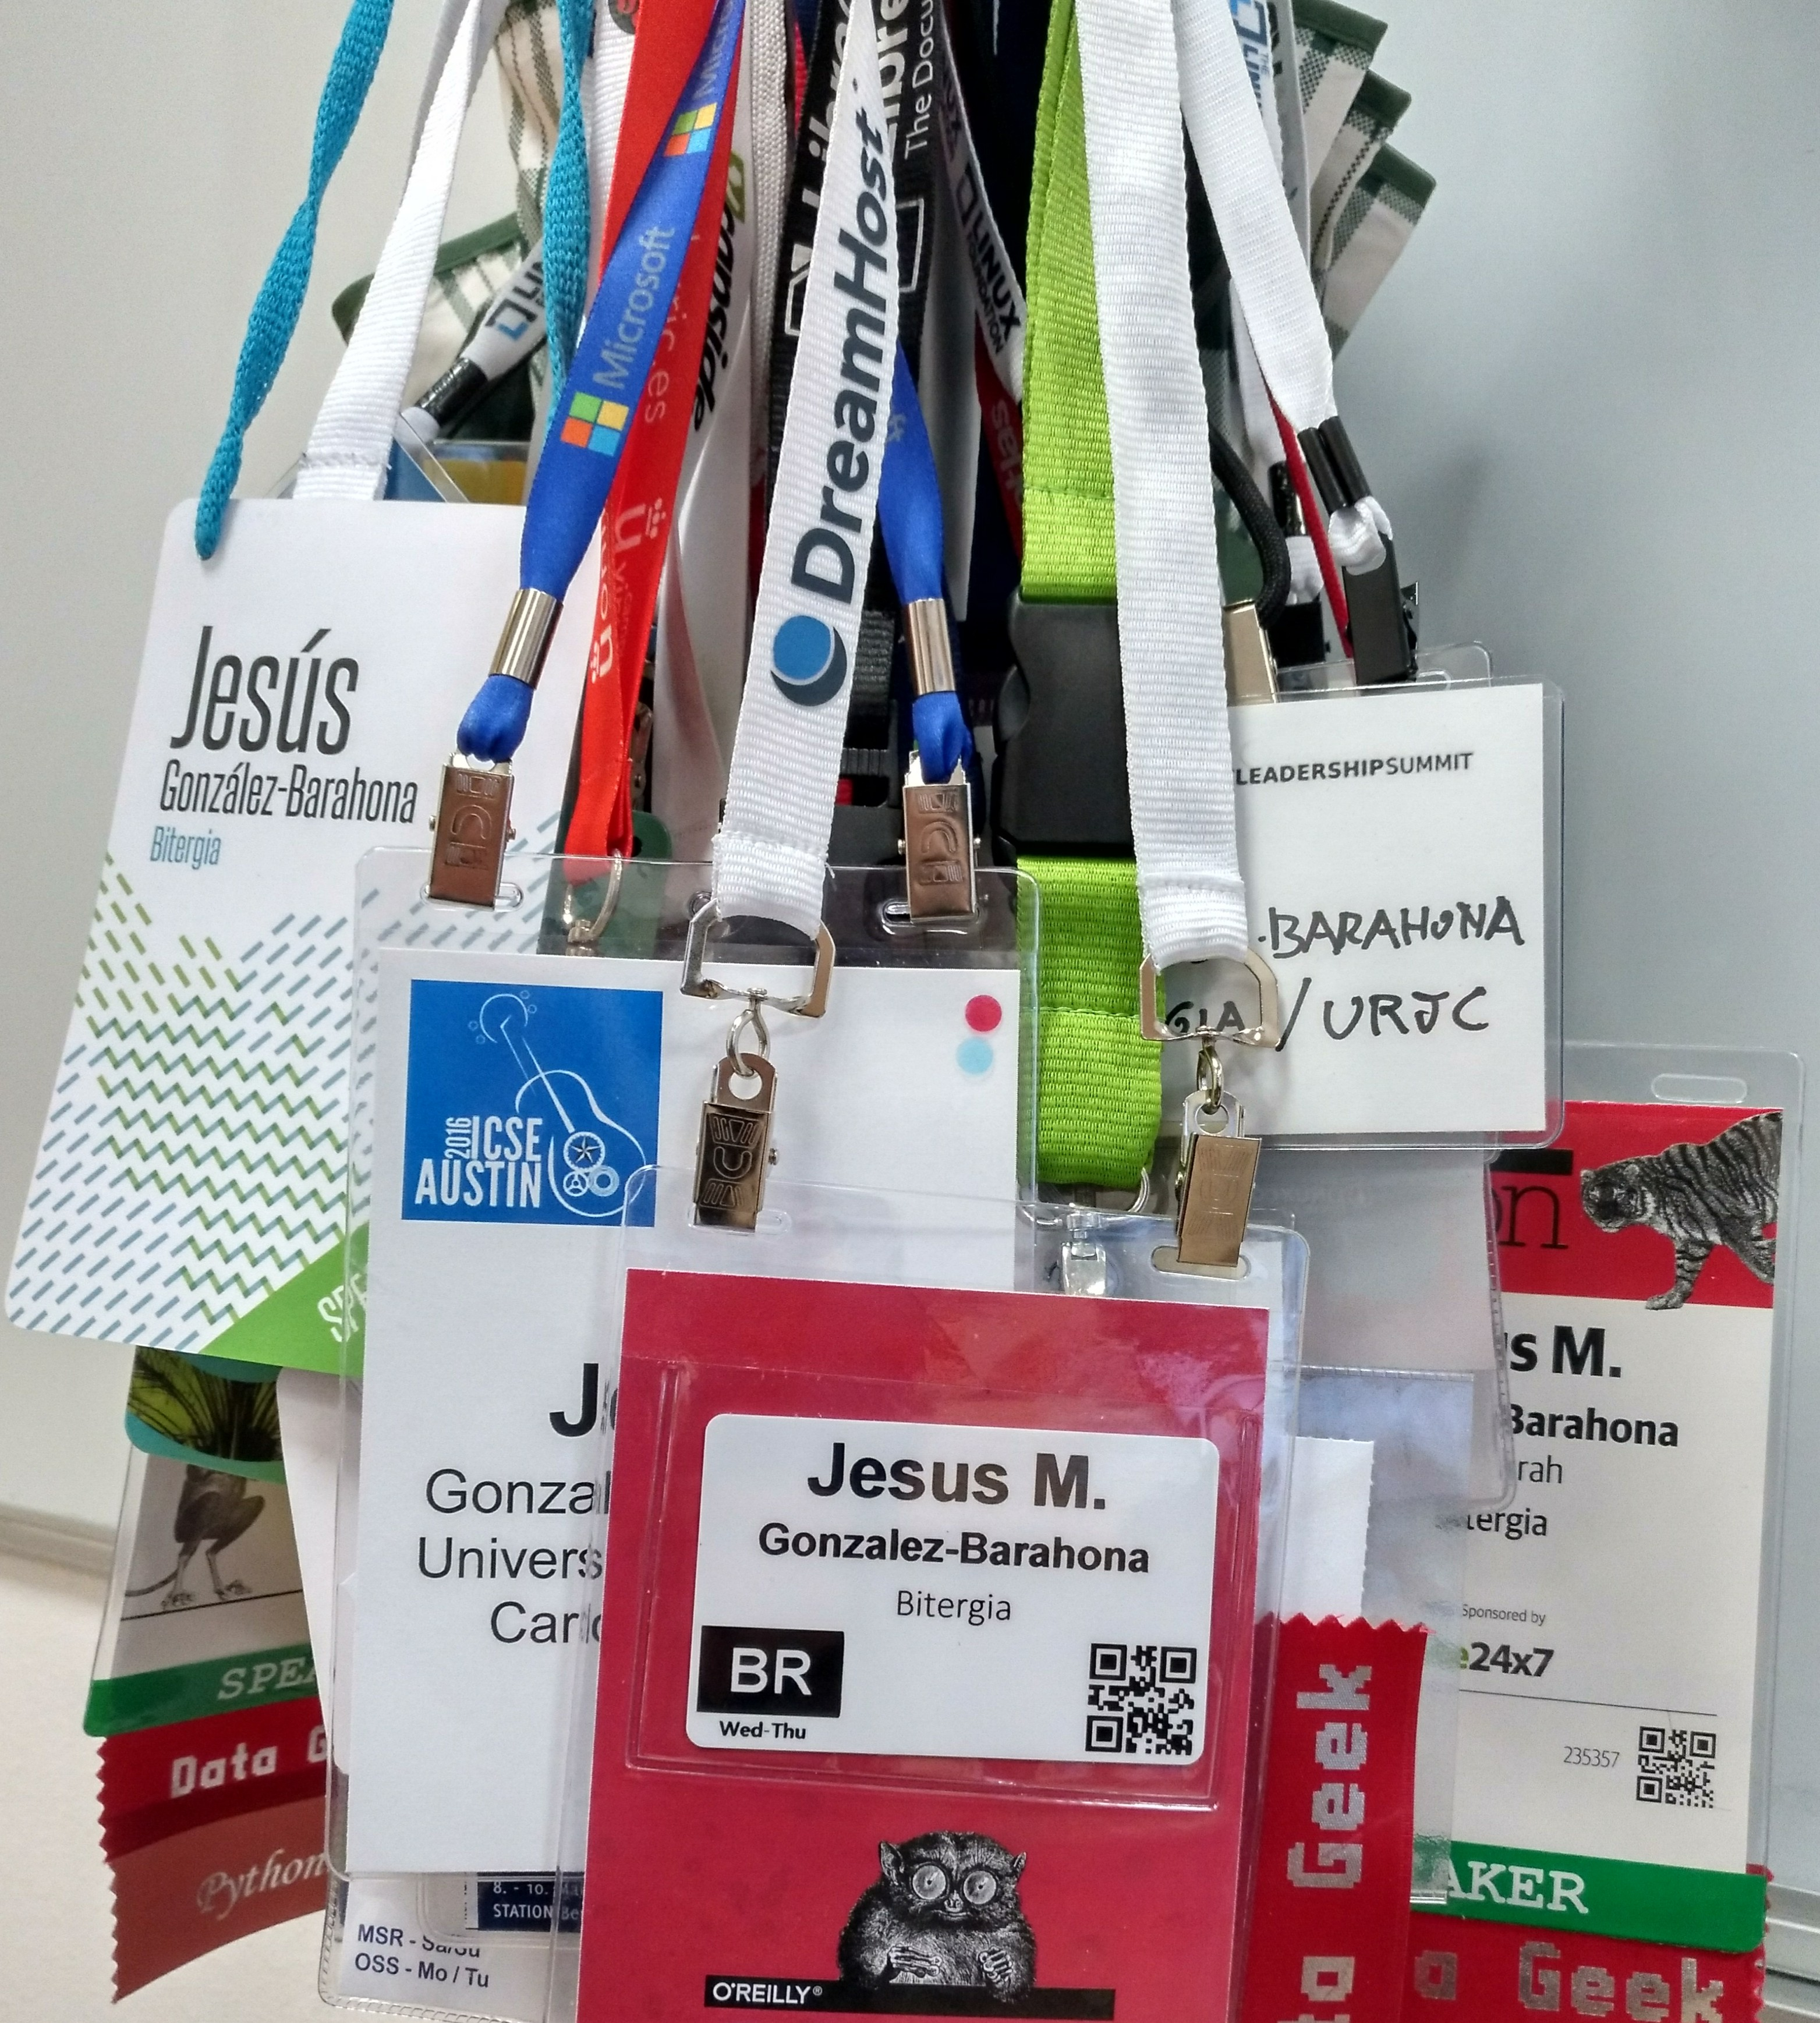
\includegraphics[width=10cm]{figs/badges}
  \end{center}  
  
\end{frame}

%%-----------------------------------------
\begin{frame}[fragile]

  \begin{center}
  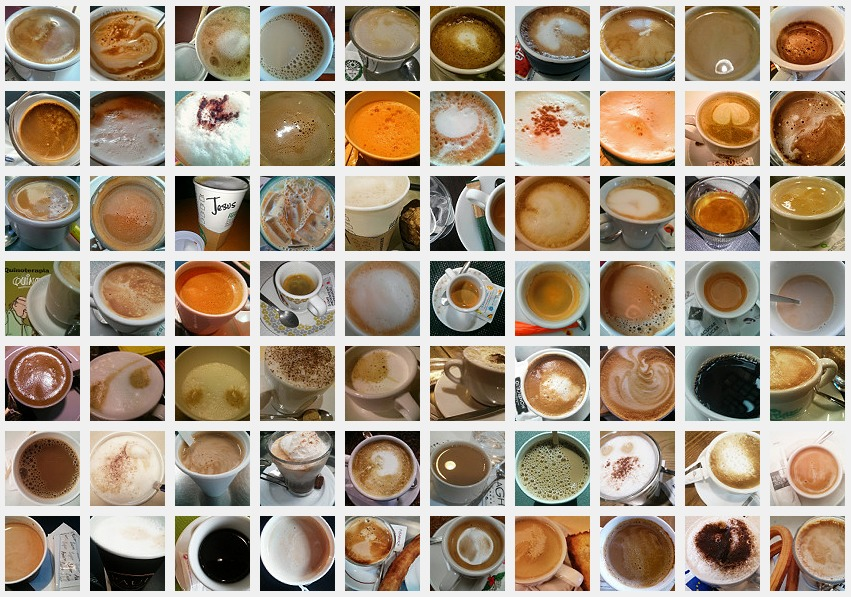
\includegraphics[width=11cm]{figs/coffees}
  \end{center}  
  
\end{frame}

%%-----------------------------------------
\begin{frame}[fragile]

  \begin{center}
    {\em \Large
      Finding a balance \\
      between having fun \\
      and having a career \\
    }
  \end{center}  
  
\end{frame}


\frame{
~
\vspace{1cm}

\begin{flushright}


\includegraphics[width=2.2cm]{figs/by-sa}
 \\

\begin{footnotesize}
\copyright 2018 Jesus M. Gonzalez-Barahona. \\

\vspace{.4cm}

Some rights reserverd. This document is distributed under the terms of the Creative Commons License ``Attribution-ShareAlike 4.0'',
available in \\
{\scriptsize \url{http://creativecommons.org/licenses/by-sa/4.0/}} \\

\vspace{.4cm}

This document (including source) is available from
\url{https://github.com/jgbarah/presentaciones}

\end{footnotesize}
\end{flushright}

}
%%

%\againframe{firstframe}

\end{document}
